%%%%%%%%%%%%%%%%%%%%%%%%%%%%%%%%%%%%%%%%%
\documentclass[paper=a4, fontsize=15pt]{article} % A4 paper and 11pt font size

\usepackage{amsmath,amsfonts,amsthm} % Math packages
\usepackage{graphicx}
\usepackage[top=0.5in, bottom=1in, left=1in, right=1in]{geometry}
\usepackage{tabularx}


\pagestyle{plain} % Makes all pages in the document conform to the custom headers and footers

\title{	
Machine Learning \\
Homework 3
}
\author{Yao Song\\301266041} % Your name
\date{\normalsize\today} % Today's date or a custom date

\begin{document}
\maketitle % Print the title
%----------------------------------------------------------------------------------------
%	PROBLEM 1
%----------------------------------------------------------------------------------------

\section*{Question 1}
\begin{align}
&\frac{\mathrm d}{\mathrm d x} \left( (1+\exp(-a)^{-1}) \right) \\
=&-(1+\exp(-a))^{-2} \frac{\mathrm d}{\mathrm d x} \left( \exp(-a) \right)\\
=& \frac{exp(-a)}{(1+\exp(-a))^{2}}\\
=& \frac{1}{1+\exp(-a)} - \frac{1}{(1+\exp(-a))^{2}}\\
=& g(a) - g(a)^2\\
=& g(a)( 1- g(a) )
\end{align}

%%%%%%%%%%%%%%%%%%%%%%%%%%%%%%%%%%%%%%%%%%%%%%%%%%%%%%%%%%%%%%%%%%%%%%%%%%%%%%%%%%

\section*{Question 2}



\section*{Question 3}

%%%%%%%%%%%%%%%%%%%%%%%%%%%%%%%%%%%%%%%%%%%%%%%%%%%%%%%%%%%%%%%%%%%%%%%%%%%%%%%%%%



\section*{Question 4}
\begin{figure}[hb]
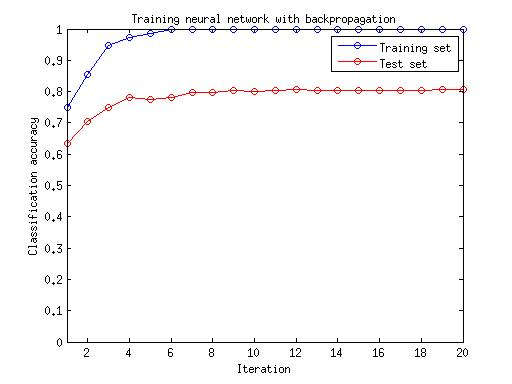
\includegraphics[width=\linewidth]{./a3_datacode/normal.jpg}
\caption{training/testing error plot}
\label{fig:normal}
\end{figure}


%%%%%%%%%%%%%%%%%%%%%%%%%%%%%%%%%%%%%%%%%%%%%%%%%%%%%%%%%%%%%%%%%%%%%%%%%%%%%%%%%%




%----------------------------------------------------------------------------------------

\end{document}